\section{Space Delay Tolerant Networks}
\label{sec:dtn}

The Delay Tolerant Networking RFC \cite{cerf2007delay} defines an architecture for irregularly connected networks subject to frequent partition and possibly long propagation delays. To face these particular properties, the authors propose an overlay layer, called the \textbf{bundle layer}, which provides end-to-end reliable messages delivery. 


\subsection{The Bundle Protocol}

The bundle layer works on the top of the transport, network or data link layer using different convergence services to communicate with lower layer protocols, Figure \ref{fig:bundle}. The Bundle protocol specification \cite{rfc5050} defines the services offered by the bundle layer, data processing format, bundle processing and convergence layers. 

\begin{figure}[ht]
\centering
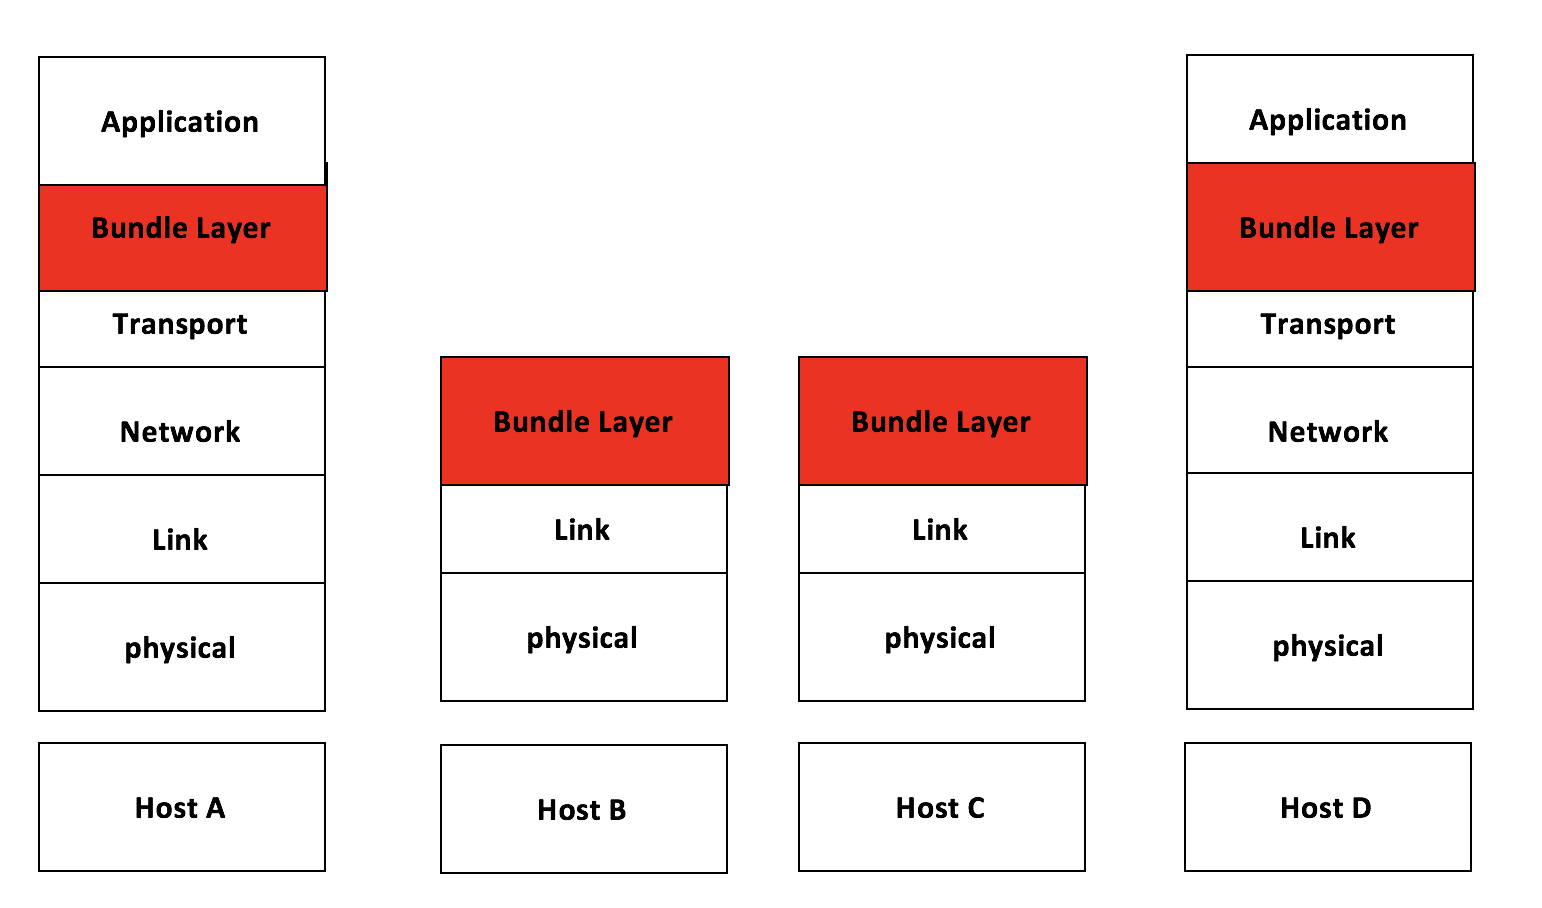
\includegraphics[width=1 \linewidth]{images/bundle.png} 
\caption{Bundle layer}
\label{fig:bundle}
\end{figure}

A bundle is the basic data unit of the Bundle protocol, similar to a packet for the IP protocol. A \textbf{bundle node}, DTN node or just simply a node could be any entity that can send or receive bundles; in other words, it is an implementation of the bundle layer. Note that a spacecraft could contain more than one instance of the Bundle protocol. For instance, the International Space Station is considered a network itself rather than a single bundle node. Negotiation between nodes might not be possible due to the delay and disruption, so a bundle is a self-contained data structure which has enough processing information.


The bundle layer provides persistent storage, hop-by-hop transfer, late binding, and optional end-to-end acknowledgement to overcome the constrained environment. The Bundle Protocol employs Universal Resources Identifiers (URI) as naming scheme, and this flexible model allows the encapsulation of different addressing schemes and late binding. 

According to CCSDS \cite{rationale2010requirements}, the Bundle protocol is the best-suited option to support in-space internetworking. There is ongoing work within the CCSDS to adapt and standardise the Bundle protocol and the security specifications. %The next section describes the security specification for the Bundle protocol. 

Many successful experiments of the Bundle protocol were already performed in deep space  \cite{ivancic2010experience}. The first experiment was conducted by Surrey Satellite Technology in 2008. The test consisted on deliver images taken by the UK-DMC Disaster Monitoring Constellation satellites to ground stations using the Bundle Protocol. Similarly, the NASA employed this protocol in the Deep Impact Space Network experiment for around four weeks on board the Deep Impact/EPOXI spacecraft. The International Space Station has been connected to the Internet since 2010 using the BP, and also performed many experiments with the NASA Jet Propulsion Labs. \cite{araniti2015contact}.    


\subsection{Security for Bundle Protocol}


 %From the beginning, the Delay-Tolerant Research Group worked on the security specifications for the Bundle protocol. The motivation was to provide data integrity and confidentiality services to the bundle layer. As space missions are more connected to the Internet and the economic value of space assets are very high is comprehensible consider information security as a critical component of the communication system.
 
 
The Bundle Security Protocol \cite{rfc6257} provides the specifications for data integrity and confidentiality services to the Bundle protocol. The document defines the data structure to provide the security services as extension blocks. A new document, still in active development \cite{ietf-dtn-bpsec-07}, defines two types of security blocks: Block Integrity Block (BIB) and Block Confidentiality Block (BCB). Previous versions of the specification define an extra security block, the Block Authentication Block BAB which was intended to provide hop-by-hop authentication but was removed in the last version of the document.     
 

Unauthorised access is a major problem for space DTNs, especially in the space segment where resources are scarce and expensive. Denial of service (DoS) is another concern; attackers could take advantage of long delays to make DoS attacks more effective \cite{rfc6257}. Sections of a space-based DTN may be untrusted, requiring encryption of payload and maybe the bundle meta-data. In the deep space, traditional mechanisms are not adequate; online access to a certificate authority cannot be assumed, and negotiation-based protocols are unsuitable.
 
 
The bundle layer operates as an overlay network; thus any vulnerability in lower layers apply to the bundle layer \cite{rfc6257}. Correspondingly, the space DTN could take advantage of security in other layers. The Bundle protocol allows a mix of ``security-aware'' nodes and ``non-security-aware'' nodes within an application domain. The lack of physical resources or security being implemented in other layers are potential scenarios for this situation. 

%\subsection{Key Management for DTN in space}
In a multi-hop communication, intermediate nodes may verify the integrity of the bundles or decrypt them according to security policies. Security-aware-nodes thus may need the corresponding verification or decryption keys, even if they are not the final destination. Key management system must contemplate this situation to fulfil the BSP.

A trade-off between usability against security is always present. Security adds overhead, but the limited resources in the space segment requires to maintain bandwidth and storage overhead low; otherwise, mission planners will reject the system. \cite{book2012architecture}.

%The next section is a literature review of the so far proposed key management solutions for DTN in space.

\subsection{Standardisation Effort}

Even though DTN working groups have been working actively since 2007, a key management specification has been postponed, mainly for its complexity \cite{rfc6257,irtf-dtnrg-sec-overview-06,templin-dtnskmps-00}. The Bundle Security Specification assumes that nodes are already in possession of shared or asymmetric key. Farrell presents high-level requirements for key management \cite{farrell-dtnrg-km-00}, but this document does not establish concluding requirements for a solution. Farrel argues that solutions must employ well-known protocols and options for manual keying, pre-shared keys, and public keys must be considered. 

The first significant advance was a problem statement by Templin in 2014  \cite{templin-dtnskmps-00}. This Internet-Draft suggests that the solution involves some type of public key cryptography and states the need for an automated system for publication of certificates and revocation lists. Templin affirmed that the system must be designed to continue the operation in the presence of long delays and intermittent connectivity, and there is no key management system which satisfies the requirements. The author suggests the use of one-time keys, so each bundle is encrypted with a symmetric key encrypted by the destination public key.  

Another more detailed Internet-Draft was published by the same author one year later \cite{templin-dtnskmreq-00}. The document proposes nine requirements for key management and four design criteria. The next section examines these requirements in detail.

Viswanathan \cite{viswanathan-dtn-pkdn-00} enumerates the possible communication patterns, data structure, architectural elements, and trust relationships.  This Internet-Draft provides a high-level solution for key distribution and revocations using the publisher/subscriber pattern. This model seems to be the best option for key distribution, assuming a key management based on public certificates. 

Finally, a newly published document proposed the Delay-Tolerant Key Administration DTKA \cite{burleigh-dtnwg-dtka-01}, which is a system for key management intended for the use in space-based DTNs. An overview of this system is presented in the next section.









